\section{包设计}
\subsection{整体架构设计}
本系统为了能更加有效地进行整合、生产宏观模型,就需要对系统中的类进行分组,以下是本系统中的包设计。
\begin{figure}[!htbp]
	\centering
	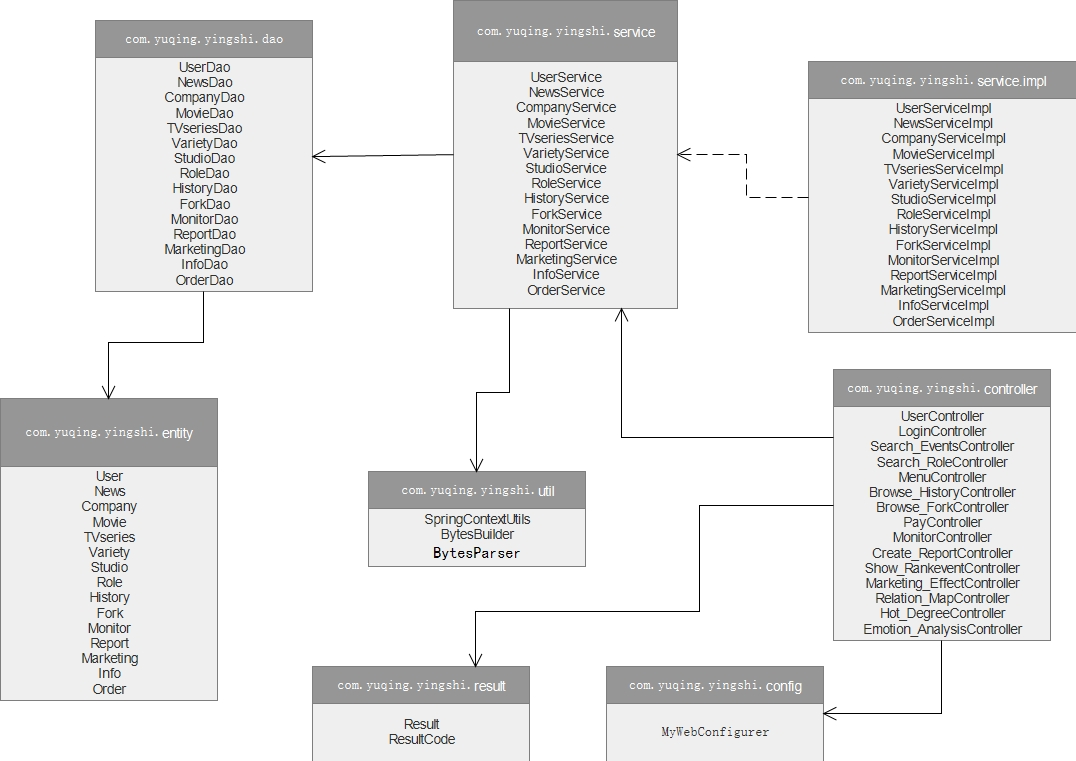
\includegraphics[scale=0.6]{image/o2.png}
	\caption{舆情系统包的设计图}
\end{figure}

\subsection{包的设计说明}
下表为服务器的包设计表
\begin{longtable}[c]{|p{6cm}|p{7cm}|}
	\caption{包设计表}
	\label{tab:tablep1}\\
	\hline
	\rowcolor[HTML]{DAE8FC} 
	包名 & 设计说明    \\ \hline
	\endfirsthead
	%
	\multicolumn{2}{c}%
	{{表13:包设计表}} \\
	\endhead
	%
	com.yuqing.yingshi.service & 该包主要存放了高层调用Dao的接口\\\hline
	com.yuqing.yingshi.controller & 改包主要存放了业务逻辑相关类,依赖于com.yuqing.yingshi.service,调用Service以完成业务逻辑\\\hline
	com.yuqing.yingshi.result& 该包存放了服务器与web端交互时返回的结果对应编码\\\hline
	com.yuqing.yingshi.dao&主要负责数据访问,该包中的类封装了对数据库的访问(只包含最原子的数据操作),供高层调用,依赖于com.yuqing.yingshi.entity\\\hline
	com.yuqing.yingshi.config& 存放了与前端web网页交互的相关配置\\\hline
	com.yuqing.yingshi.entity&该包主要存放数据库表中所对应的实体类\\\hline
	com.yuqing.yingshi.service.impl&该包存放了service包中定义的接口的具体实现\\\hline
	com.yuqing.yingshi.util&存放了项目相关工具类\\\hline
\end{longtable}

\section{类设计}
本小结以包为单位,对每个包所含有的类及类与类间的调用关系进行说明。

\begin{table}
	\caption{com.yuqing.yingshi.dao相关类}
	\centering
	\begin{tabular}{|p{3cm}|p{10cm}|} 
		\hline 
		\rowcolor[HTML]{DAE8FC} 
		\multicolumn{2}{|c|}{com.yuqing.yingshi.dao相关类} \\ 
		\hline 
		UserDao&封装与User实体类相关的数据访问方法\\
		NewsDao&封装与News实体类相关的数据访问方法\\
		CompanyDao&封装与Company实体类相关的数据访问方法\\
		MovieDao&封装与Movie实体类相关的数据访问方法\\
		TVseriesDao&封装与TVseries实体类相关的数据访问方法\\
		VarietyDao&封装与Variety实体类相关的数据访问方法\\
		StudioDao&封装与Studio实体类相关的数据访问方法\\
		RoleDao&封装与Role实体类相关的数据访问方法\\
		HistoryDao&封装与History实体类相关的数据访问方法\\
		ForkDao&封装与Fork实体类相关的数据访问方法\\
		MonitorDao&封装与Monitor实体类相关的数据访问方法\\
		ReportDao&封装与Report实体类相关的数据访问方法\\
		MarketingDao&封装与Marketing实体类相关的数据访问方法\\
		InfoDao&封装与Info实体类相关的数据访问方法\\
		OrderDao &封装与Order实体类相关的数据访问方法\\
		\hline 
	\end{tabular}
\end{table}



\begin{table}
	\caption{com.yuqing.yingshi.entity相关类}
	\centering
	\begin{tabular}{|p{3cm}|p{10cm}|} 
		\hline 
		\rowcolor[HTML]{DAE8FC} 
		\multicolumn{2}{|c|}{com.yuqing.yingshi.entity相关类} \\ 
		\hline 
		User &用户个人信息的实体类\\
		News &新闻信息的实体类\\
		Company &公司信息的实体类\\
		Movie&电影信息的实体类\\
		TVseries&影视剧信息的实体类\\
		Variety&综艺信息的实体类\\
		Studio&工作室信息的实体类\\
		Role&演员/歌手等明星信息的实体类\\
		History&历史记录的实体类\\
		Fork&收藏记录的实体类\\
		Monitor&监控预警项的实体类\\
		Report&报告的实体类\\
		Marketing&营销效果的实体类\\
		Info &单条博文/帖子信息的实体类\\
		Order &用户订单的实体类\\
		\hline 
	\end{tabular}
\end{table}




\begin{table}
	\caption{com.yuqing.yingshi.service相关类}
	\centering
	\begin{tabular}{|p{3cm}|p{10cm}|} 
		\hline 
		\rowcolor[HTML]{DAE8FC} 
		\multicolumn{2}{|c|}{com.yuqing.yingshi.service相关类} \\ 
		\hline 
		UserService&定义了与User实体类相关的业务逻辑接口\\
		NewsService&定义了与News实体类相关的业务逻辑接口\\
		CompanyService&定义了与Company实体类相关的业务逻辑接口\\
		MovieService&定义了与Movie实体类相关的业务逻辑接口\\
		TVseriesService&定义了与TVseries实体类相关的业务逻辑接口\\
		VarietyService&定义了与Variety实体类相关的业务逻辑接口\\
		StudioService&定义了与Studio实体类相关的业务逻辑接口\\
		RoleService&定义了与Role实体类相关的业务逻辑接口\\
		HistoryService&定义了与History实体类相关的业务逻辑接口\\
		ForkService&定义了与Fork实体类相关的业务逻辑接口\\
		MonitorService&定义了与Monitor实体类相关的业务逻辑接口\\
		ReportService&定义了与Report实体类相关的业务逻辑接口\\
		MarketingService&定义了与Marketing实体类相关的业务逻辑接口\\
		InfoService&定义了与Info实体类相关的业务逻辑接口\\
		OrderService&定义了与Order实体类相关的业务逻辑接口\\
		\hline 
	\end{tabular}
\end{table}
\begin{table}
	\caption{com.yuqing.yingshi.util相关类}
	\centering
	\begin{tabular}{|p{4.5cm}|p{8.5cm}|} 
		\hline 
		\rowcolor[HTML]{DAE8FC} 
		\multicolumn{2}{|c|}{com.yuqing.yingshi.util相关类} \\ 
		\hline 
		SpringContextUtils&获取spring容器bean对象工具类\\
		BytesBuilder&字节构造器\\
		BytesParser&字节处理器\\
		\hline 
	\end{tabular}
\end{table}
\begin{table}
	\caption{com.yuqing.yingshi.result相关类}
	\centering
	\begin{tabular}{|p{4.5cm}|p{8.5cm}|} 
		\hline 
		\rowcolor[HTML]{DAE8FC} 
		\multicolumn{2}{|c|}{com.yuqing.yingshi.result相关类} \\ 
		\hline 
		Result&结果返回形式定义\\
		ResultCode&定义返回结果编码\\
		\hline 
	\end{tabular}
\end{table}
\begin{table}
	\caption{com.yuqing.yingshi. controller相关类}
	\centering
	\begin{tabular}{|p{4.5cm}|p{8.5cm}|} 
		\hline 
		\rowcolor[HTML]{DAE8FC} 
		\multicolumn{2}{|c|}{com.yuqing.yingshi. controller相关类} \\ 
		\hline 
		UserControlle&定义了响应用户相关界面不同点击事件的方法,根据事件的不同调用 UserService的相应方法实现功能,以json格式返回。\\
		LoginController&定义了登陆注册界面不同点击事件的方法,根据事件的不同调用 UserService的相应方法实现功能,以json格式返回。\\
		Search\_EventsController&定义了搜索热门影视事件/影视作品相关界面不同点击事件的方法,根据事件的不同调用 NewsService、MovieService、TVseriesService、VarietyService的相应方法实现功能,以json格式返回。\\
		Search\_RoleController&定义了搜索明星/公司/工作室相关界面不同点击事件的方法,根据事件的不同调用 RoleService、CompanyService、StudioService的相应方法实现功能,以json格式返回。\\
		MenuController&定义了展示影视事件/明星/影视作品菜单相关界面不同点击事件的方法,根据事件的不同调用 RoleService、CompanyService、StudioService、NewsService、MovieService、TVseriesService、VarietyService的相应方法实现功能,以json格式返回。\\
		Browse\_HistoryController&定义了浏览历史记录相关界面不同点击事件的方法,根据事件的不同调用 HistoryService的相应方法实现功能,以json格式返回。\\
		Browse\_ForkController&定义了浏览收藏记录相关界面不同点击事件的方法,根据事件的不同调用 ForkService的相应方法实现功能,以json格式返回。\\
		\hline 
	\end{tabular}
\end{table}


\newpage
\section{接口设计}
\subsection{外部接口设计}
外部接口是各模块间进行交互访问以及web访问系统时的外部接口,某一模块的具体功能则由内部接口设计实现。
\begin{figure}[!htbp]
	\centering
	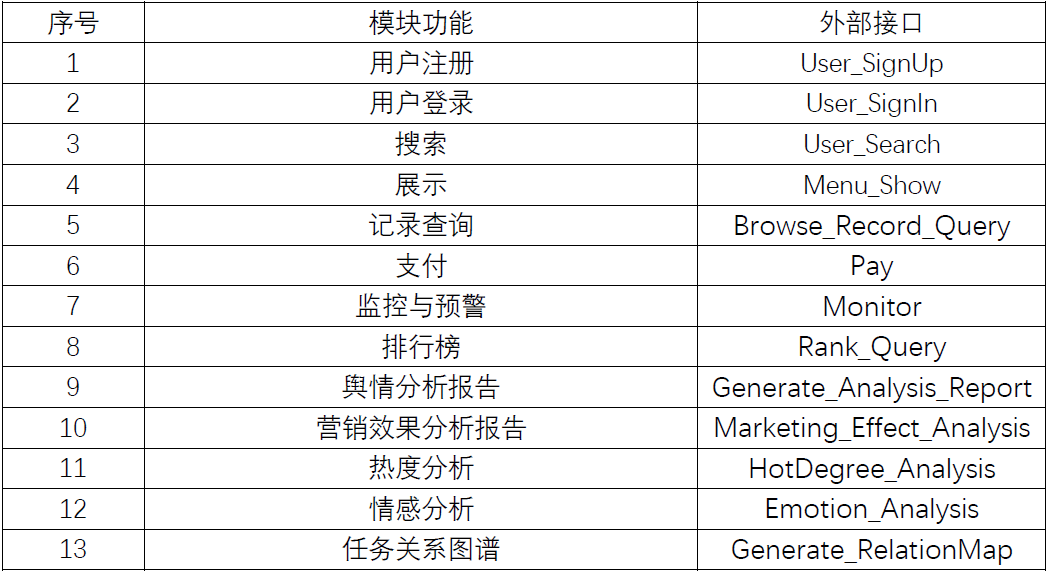
\includegraphics[scale=0.7]{image/m1.png}
	\caption{外部接口设计}
\end{figure}
\subsection{内部接口设计}
\subsubsection{注册登录模块}
\begin{figure}[!htbp]
	\centering
	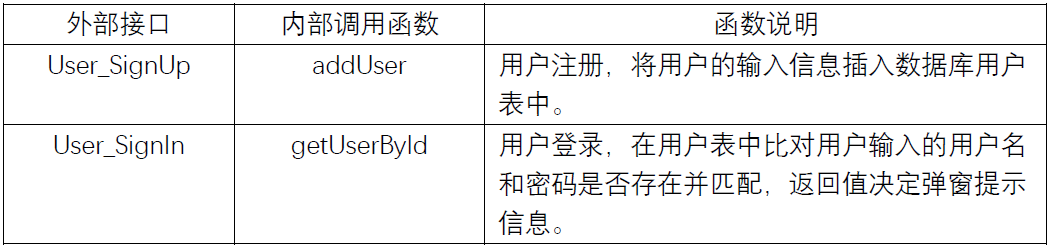
\includegraphics[scale=0.7]{image/m2.png}
	\caption{注册登录模块}
\end{figure}
\subsubsection{搜索模块}
\begin{figure}[!htbp]
	\centering
	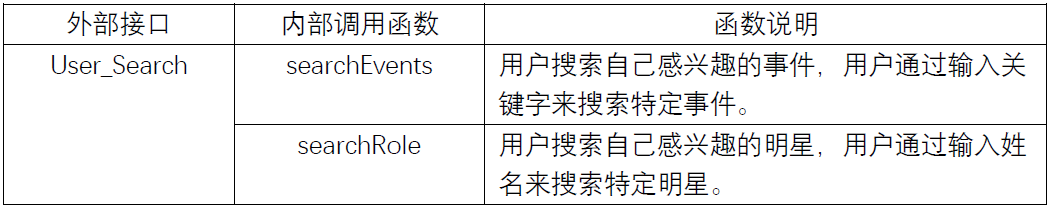
\includegraphics[scale=0.7]{image/m3.png}
	\caption{搜索模块}
\end{figure}
\subsubsection{展示模块}
\begin{figure}[!htbp]
	\centering
	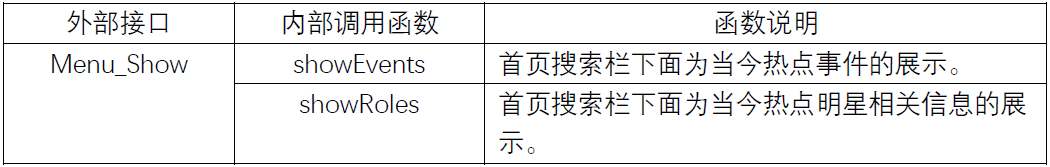
\includegraphics[scale=0.7]{image/m4.png}
	\caption{展示模块}
\end{figure}
\subsubsection{记录查询模块}
\begin{figure}[!htbp]
	\centering
	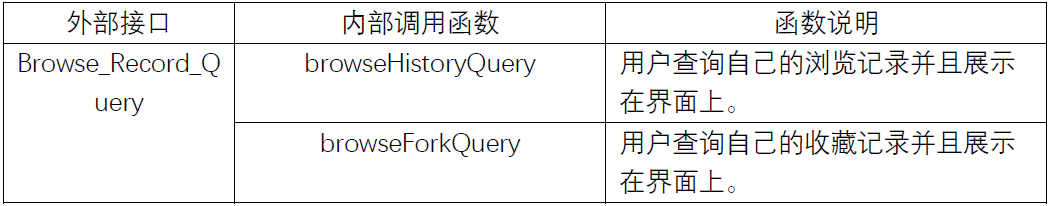
\includegraphics[scale=0.7]{image/m5.png}
	\caption{记录查询模块}
\end{figure}
\subsubsection{支付模块}
\begin{figure}[!htbp]
	\centering
	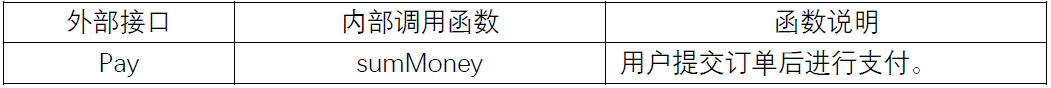
\includegraphics[scale=0.7]{image/m6.png}
	\caption{支付模块}
\end{figure}
\subsubsection{监控与预警模块}
\begin{figure}[!htbp]
	\centering
	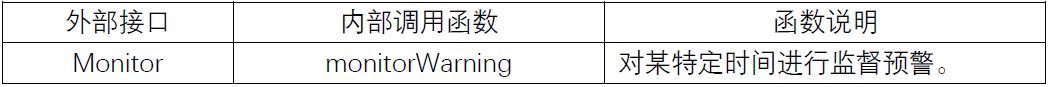
\includegraphics[scale=0.7]{image/m7.png}
	\caption{监控与预警模块}
\end{figure}
\subsubsection{排行榜模块}
\begin{figure}[!htbp]
	\centering
	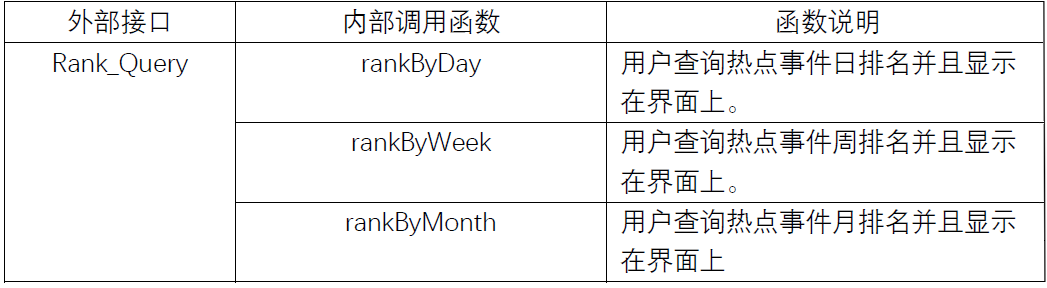
\includegraphics[scale=0.55]{image/m8.png}
	\caption{排行榜模块}
\end{figure}
\subsubsection{分析模块}
\begin{figure}[!htbp]
	\centering
	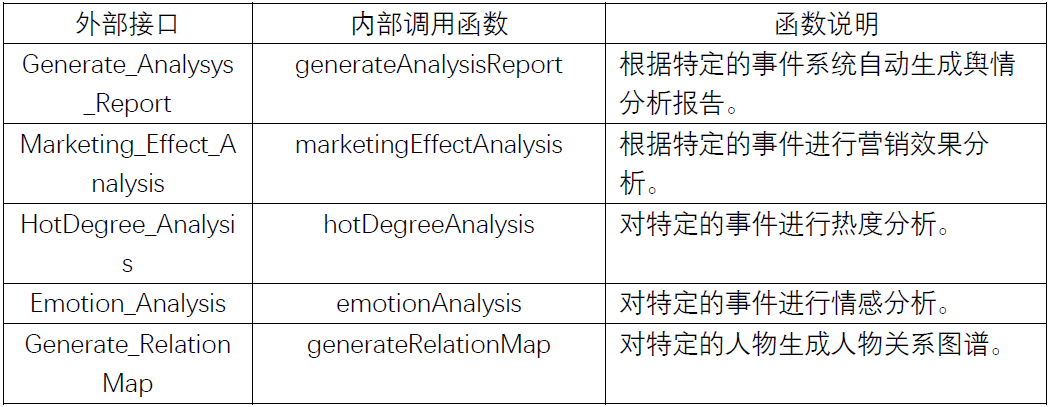
\includegraphics[scale=0.7]{image/m9.png}
	\caption{分析模块}
\end{figure}
